\documentclass[10pt]{llncs}

% T1 fonts used to generate the final print and online PDFs
\usepackage[T1]{fontenc}
\usepackage{geometry}
\usepackage{graphicx}

% uncomment these if using hyperref package to display URLs in blue roman font
%\usepackage{color}
%\renewcommand\UrlFont{\color{blue}\rmfamily}

% picture overlay (title page)
\usepackage[percent]{overpic}

\usepackage[nottoc,section]{tocbibind}

% define new colors
\usepackage[dvipsnames]{xcolor}

\newenvironment{acknowledgement}{%
      \list{}{\advance\topsep by0.35cm\relax
      \leftmargin=1cm
      \labelwidth=0cm
      \listparindent=0cm
      \itemindent\listparindent
      \rightmargin\leftmargin}\item[\hskip\labelsep
        \bfseries\ackname]}
% Defines a new environment for acknowledgements.

\renewenvironment{abstract}{%
      \list{}{\advance\topsep by0.35cm\relax
      \leftmargin=1cm
      \labelwidth=0cm
      \listparindent=0cm
      \itemindent\listparindent
      \rightmargin\leftmargin}\item[\hskip\labelsep
        \bfseries\abstractname]}
% Overwrites environment for the abstract.

\setcounter{tocdepth}{3}
% Used to define table of contents.

\geometry{
  textwidth=12.2cm,  % llncs has 12.2cm
  textheight=19.3cm, % llncs has 19.3cm
  centering
}
% Used to define the margins of the pages.

\pagestyle{headings}
% Used for page numbering.

\usepackage{hyperref}
% Used for hyperlinking cross-referenced elements.

\makeatletter
\renewcommand\subsubsection{\@startsection{subsubsection}{3}{\z@}%
                       {-18\p@ \@plus -4\p@ \@minus -4\p@}%
                       {12\p@ \@plus 4\p@ \@minus 4\p@}%
                       {\normalfont\normalsize\bfseries\boldmath
                        \rightskip=\z@ \@plus 8em\pretolerance=10000}}
\renewcommand\paragraph{\@startsection{paragraph}{4}{\z@}%
                       {-18\p@ \@plus -4\p@ \@minus -4\p@}%
                       {12\p@ \@plus 4\p@ \@minus 4\p@}%
                        {\normalfont\normalsize\itshape
                        \rightskip=\z@ \@plus 8em\pretolerance=10000}}
\makeatother
% Used for reformatting heading level 3 and 4


\begin{document}
%
%Start
\newgeometry{textheight=700pt,top=50pt,left=50pt,right=50pt}
\begin{titlepage}
%\vspace*{0.8cm}
\begin{figure}[h]{%
      \includegraphics[width=0.4\textwidth]{Logo.png}
    }
\end{figure}

\vspace*{2cm}

%%%% Add the title of your thesis here
{\Huge  \textbf{Explainability Methods for Dynamic Graphs}}

\vspace*{0.5cm} 

{\Large Group report}

%\vspace*{6.5cm}
{\raggedleft\vfill{%

%
% ---- Write your names here ----
%
% In case of groups of two students:
% 1. Change \begin{tabular}{c c c} to \begin{tabular}{c c}
% 2. Delete  & {\Large Name 3}
% 3. Delete  & {Student number 3} 
\setlength{\tabcolsep}{12pt}
\begin{tabular}{c c c}
        {\Large Name 1}  &  {\Large Name 2} & {\Large Name 3} \\
        {Student number 1}  & {Student number 2} & {Student number 3} 
\end{tabular}
\linebreak
\vspace*{1.5cm}


\textbf{{\large Thesis submitted to obtain \linebreak
the degree of}} \linebreak

%!!!IMPORTANT!!!:
%indicate the appropriate title of your master and major. Check the website https://feb.kuleuven.be/studentenportaal/contact/masterproef-leuven
{\large Master of Information Management}\linebreak
%In case of master thesis in Dutch, use the line below
%{\large Master in het informatiemanagement}\linebreak
%{\large Major Data science }\linebreak
\linebreak
\textbf{{\large Promoter:}}   Prof.\ Dr.\ ... \linebreak
\textbf{{\large Daily Supervisor:}}  ... \linebreak

%\linebreak

\textbf{{\large Academic year:}} {\large 20XX-20XX}
\linebreak
}\par}

\end{titlepage}
\restoregeometry
\clearpage

%%%%%%%%%%%%%%%%%%%%%%%%%%%%%%%%%%%%%%%%%%%%%%%%%%%%%%%%%%%%%%%%%%%%%%%%%%%%%%%%%%%%%%%%%%%%%%%%%%%% 

\restoregeometry

%
% ---- Abstract ----
%
\normalsize\begin{abstract} \normalsize
The abstract should briefly summarize the contents of the paper in
150--250 words.

\keywords{First keyword  \and Second keyword \and Another keyword.}
\end{abstract}
\clearpage
%
\restoregeometry

%
% ---- Acknowledgements ----
%
\begin{acknowledgement} \input{Content/0_Acknowledgements.tex}
\end{acknowledgement}
\clearpage
%
%
% ---- Table of contents ----
%
\tableofcontents

\clearpage

%
% ---- Introduction ----
%
\section{Introduction} 

Dynamic graphs have become increasingly popular in recent years as they provide a flexible and powerful framework for representing complex systems that evolve over time. These graphs have applications in a wide range of fields, from social networks to biological systems, and are used to model the interactions and relationships between different entities. However, as dynamic graphs become more complex, understanding and interpreting them can be challenging. Explainability, or the ability to understand why a particular result or decision was reached, is crucial for many applications, including fraud detection, recommendation systems, and predictive analytics. Despite the growing importance of explainability in dynamic graphs, there is a lack of comprehensive surveys in the field. This survey aims to fill this gap by exploring the state of the art in explainability in dynamic graphs and identifying key challenges and opportunities for future research.


\subsection{Graph description}
A dynamic graph is a mathematical structure that evolves over time, with the appearance and removal of edges and nodes. It is a type of graph that captures the dynamic nature of real-world systems, where relationships between entities may change over time. In a dynamic graph, edges and nodes are not static and can change their state or disappear over time. For example, social networks can be represented as dynamic graphs, where the nodes are people and the edges are the relationships between them, such as friendships or collaborations.

On the other hand, a temporal graph is a static graph where the nodes and edges have attributes that change over time. In this case, the topology of the graph is fixed, but the properties of the nodes and edges vary over time. For instance, a transportation network can be represented as a temporal graph, where the nodes are locations, and the edges are roads or routes connecting them. The attributes of nodes and edges could include travel time, congestion, or availability, which change over time.

To illustrate the difference between dynamic graphs and temporal graphs, consider a network of mobile phone calls between people. A dynamic graph would track the creation and deletion of calls between individuals, while a temporal graph would capture the evolution of the duration, frequency, and location of these calls.

In this paper, we propose to distinguish between dynamic and temporal graphs based on the definition that a dynamic graph refers to the appearance and removal of edges and nodes, while a temporal graph refers to the evolution of features. We also suggest that static graphs with temporal features should be referred to as temporal graphs, while dynamic graphs with static features should be called dynamic graphs. In other words, the time variation of edges and node is called 'dynamic', while it is called 'temporal' for features. Moreover, if not specified, staticness is assumed.

\subsection{Explainability vs Interpretability}

Explainability refers to the post-hoc analysis of black boxes, meaning that the model is treated as a "black box" whose inner workings are not initially understood, but after the model generates output, explanations are derived to understand the reasoning behind the output. The explanation process is done after the fact, rather than during the model's development. In contrast, interpretability refers to the intrinsic human understandable model, meaning that the model is transparent and interpretable from the outset. Interpretability involves understanding the model's design and operation, and how its components interact to produce output.\cite{trustworthy}

On the other hand, interpretability in GNNs refers to the ability to understand how the model operates and how its components interact. This can be achieved by using interpretable architectures, such as graph convolutional networks (GCNs), that allow for a more intuitive understanding of the model's behavior.

In summary, while explainability involves understanding a model's output after it is generated, interpretability refers to the ability to understand the model's inner workings and design from the outset. Both are essential in graph and network analysis, particularly in the context of complex models such as dynamic GNNs. We will use the term explanation as a combination of explanability and interpretability.

The distinction between interpretability and explainability is not always clear-cut, and the terms are often used interchangeably.  For instance, attention mechanisms. They are sometimes referred as interpretability and sometimes as explainability. In this paper, we place it as interpretability since even though it give post-hoc explanation, the weights are calulated during the detection training and are intrinsacally linked to the prediction model.



Dynamic graph and dynamic explainability being very novel domains, a common vocabulary and structure as yet to appear. Most of the papers appeared in Summer 2022. For this reason, we proposed the above definitions to facilitate future work.

\subsection{Accuracy vs. explanation}
The application of machine learning techniques to the domain of algorithmic anomaly detection (e.g., fraud detection) has created the need for additional explanatory layers to interpret and verify results. Traditional, non-deep learning anomaly detection methods transform graph data transparently, but struggle to effectively capture and represent their more complex and interdependent features. Deep learning algorithms provide a scalable and robust alternative at the cost of interpretability, operating as black boxes. The field of ‘explainability’ attempts to remedy this through analysis of deep learning model characteristics but has been largely constrained to static graphs.

\subsection{Embedding approach}
Approaches for analyzing dynamic graphs usually build upon those for static graphs, but with added consideration for temporal dimensions and update methods. For instance, matrix factorization-based methods rely on eigenvectors of the graph Laplacian matrix to generate node embeddings, which can be updated efficiently using prior embeddings in DANE. Meanwhile, random walk-based approaches use the inner products of node embeddings to model transition probabilities conditioned on history, such as in CTDANE and NetWalk. The wave of deep learning has also introduced unsupervised and supervised methods, such as DynGEM, which is an autoencoding approach that minimizes the reconstruction loss and uses an adaptive architecture depth that is initialized with previous time steps. Another category is point processes that are continuous in time, like KnowEvolve and DyRep, which model the occurrence of an edge as a point process and use neural networks to parameterize the intensity function. Combinations of graph neural networks (GNNs) and recurrent architectures, such as LSTM, have also been explored, particularly with graph convolutional networks (GCNs), as seen in GCRN, WD-GCN/CD-GCN, RgCNN, and STGCN. These approaches use graph convolution layers to modify the LSTM or perform spatiotemporal convolutions for evolving node features. STGCN was specifically designed for spatiotemporal traffic data using graph convolutions to handle spatial information.\cite{egcn}



Review that focuses on deep learning models that are designed to handle data with both temporal and spatial components exists. These models are typically created by combining existing neural network layers designed for sequential and static graph-structured data.

Temporal deep learning involves generating in-memory representations of data points using techniques such as LSTM and GRU. These representations are iteratively updated as new data is processed. Alternatively, some temporal deep learning models use an attention mechanism to adaptively re-contextualize representations based on the temporal history of the data.

The second type of model, known as static graph representation learning, involves learning representations of vertices, edges, and whole graphs using graph neural networks. This is done by generating compressed representations (messages) of node and edge attributes, which are propagated between nodes based on a message-passing rule and then aggregated to form new representations. Several existing graph neural network architectures fit this general description, differing mainly in their assumptions about the input graph and the specific compression, propagation, and aggregation functions they use.

Finally, spatiotemporal deep learning models combine the basic ideas of temporal deep learning and graph representation learning to work with temporal graph sequences. These models perform message-passing at each time point using a graph neural network block and incorporate new temporal information using a temporal deep learning block. By doing so, these models can take advantage of the shared temporal and spatial autocorrelation information across spatial units. The temporal and spatial layers of these models are fused together in a single parametric machine learning model that is trained jointly, exploiting the end-to-end differentiability of the fused models. Table 1 summarizes the spatiotemporal deep learning models we have implemented in our framework, categorized based on the type of temporal and graph neural network layer blocks used, as well as the order of spatial proximity and heterogeneity of the edge set.\cite{rozemberczki2021pytorch}




\clearpage

%
% ---- Literature Review ----
%
\section{Literature Review}
This literature review's focus is on anomaly detection and explanation in dynamic graphs. The review is divided into four parts, one covering literature on fraud and anomaly detection in static and dynamic graphs respectively and the others focusing on literature related to explanation in static and dynamic graphs. This division is due to the fact that the original purpose of the research was to explore explainability in the context of anomaly detection in dynamic graphs. However, it was found that there is limited literature available on this topic, which led to the division of the literature review into three distinct parts. This literature review aims to provide a detailed analysis of the current research trends and gaps.
It is important to note that knowledge graphs aren't included in this paper. In fact, due to their different nature , knowledge graph explanability is already widely explored in static and dynamic context.

\subsection{GNN Fraud explanation in static graphs}
One key difference between anomaly detection and classification in dynamic graphs is the nature of the problem being solved. In anomaly detection, the goal is to identify rare or unexpected events that deviate from the norm, whereas in classification, the goal is to assign a label or category to each node or edge based on its properties. Anomaly detection is therefore a more complex problem, as it involves identifying patterns that are not easily discernible from the underlying data.

Another difference is the set of constraints that come with anomaly detection. Since anomalies are by definition rare or unexpected events, they may not be well-represented in the training data. This means that anomaly detection algorithms may need to be designed to work with limited or incomplete data, and to be robust to noisy or unreliable data. Because of these differences, classification models need to be adapted for anomaly detection.

Libraries like DIG and PyGOD libraries, which have gained popularity in recent years due to their ability to provide efficient and reliable anomaly detection algorithms. DIG, which stands for Dive into Graphs. Similarly, PyGOD, which stands for Python Graph-based Outlier Detection, is another library that provides graph-based approaches for anomaly detection. 

Anomaly detection and fraud detection are related but distinct problems. In fraud detection camouflage is considered as the norm. Camouflage is a technique used by fraudsters to hide their fraudulent activities. For example, in a financial transaction network, a fraudster may try to hide their fraudulent transactions by making them appear similar to legitimate transactions.

The cost of false positives and false negatives in anomaly detection and fraud detection can be significant. A false positive occurs when a normal data point is flagged as anomalous or fraudulent, while a false negative occurs when an anomalous or fraudulent data point is not flagged. False positives can lead to unnecessary investigations or actions, while false negatives can result in missed opportunities to detect and prevent fraud. The cost of false positives and false negatives will depend on the specific application and context. Having a cost aware detection model is key in Financial systems. However few are the papers that focuses on cost for the Bank. This is a possible future direction.



\begin{table}
\caption{GNN Fraud detection and explanation in static graphs}\label{tab1}
\begin{tabular}{|l|l|l|l|l|}
\hline
Paper &  Year & Technique & Explanability type & Learning\\
\hline
Rao et al.\cite{xfraud} &  2021 & xFraud & Perturbation & Supervised\\
Qin et al.\cite{NGS} &  2022 & NGS  & Perturbation& Supervised\\
Viloria et al.\cite{RAP} & 2021 & GNNExplainer & Perturbation& Supervised\\
 WU et al.\cite{DEDGAT}& 2023 & DEDGAT & Perturbation& Supervised\\
\hline
\end{tabular}
\end{table}

The success of perturbation in fraud detection and explanation is important to note. According to a study by GraphFrameX \cite{graphframex}, their systematic evaluation framework was tested on a production use case, which was to explain fraudulent transactions in the e-commerce scenario at eBay. The study only focused on explaining correct predictions and found that GNNexplainer was the most effective method, returning both sufficient and necessary explanations. Unlike other methods, GNNExplainer computes edge and node features importance independently when solving the optimization problem, which explains its superiority in this case. The study also revealed that perturbation-based methods outperformed structure-based and gradient-based methods in this particular production use case. 

It is dangerous to solely rely on supervised techniques for anomaly detection with GNNs (Graph Neural Networks) because these models are only as good as the data they are trained on. Supervised techniques require labeled data, which means data with a clear indication of what is anomalous and what is not. However, in many cases, anomalous data may not be present in the training data, making it difficult for the model to accurately identify anomalous data in the real world. Unsupervised fraud detection and explanation using GNN in static graph is very challenging but would yield interesting results.

Note these paper are fraud specific but other broader anomaly detection technique can also work for fraud detection.

\subsection{GNN Anomaly detection in dynamic graphs}

In addition to topological and feature information, temporal data is also present in dynamic graphs. This can be very informative but is chanllenging to use. To address this challenge, dynamic GNNs typically use temporal convolutions, recurrent neural networks (RNNs), or attention mechanisms to incorporate temporal information into the model. These techniques allow the model to capture the temporal dependencies between nodes and to predict future states of the graph.

Pytorch geometric temporal (PyGT) \cite{rozemberczki2021pytorch} is an open-source library built on top of PyTorch Geometric, which is a popular library for deep learning on graphs. PyGT extends the capabilities of PyTorch Geometric to temporal graphs by providing a set of modules that enable the handling of graph sequences, i.e., a series of graphs that evolve over time. These modules allow for the creation of neural network models that can learn temporal patterns in the graph sequences, enabling tasks such as node classification, link prediction, and graph classification.


\begin{table}
\caption{Anomaly detection in dynamic graphs}\label{tab1}
\begin{tabular}{|l|l|l|l|l|l|}
\hline
Paper &  Year & Technique & detection & code & Learning\\
\hline
Zheng et al.\cite{addGraph} & 2019 & addGraph & edge & yes & semi-supervised\\
Li et al.\cite{dynWatch} & 2022 & DynWatch  & edge & yes & supervised\\
Jiang et al.\cite{TSAD} & 2022 & TSAD & community & no & supervised\\
& & TADDY &  & & \\
 & & T2EG &  & & \\
 & & DyHGN &  & & \\
 & & StrGNN &  & & \\
 & & DynAD &  & & \\
 & & ... &  & & \\
 & &  &  & & \\
\hline
\end{tabular}
\end{table}

This is not a comprehensive list since there is too many papers on the topic. However survey on Anomaly detection in dynamic graphs with a clear structure would be of great help to the current literature. Some sureys like https://arxiv.org/pdf/2209.14930.pdf or https://www.sciencedirect.com/science/article/pii/S0166361521001056 did a partial work in the huge sorting problem that a global survey on GNN anomlay detection in dynamic graph would be.

Note these paper are anomaly specific but other broader classification technique like EvolveGCN\cite{egcn} can also work for anomaly detection in dynamic graphs.

\subsection{Explanation Survey's for static graphs}
Explanation in static graphs is already widely explored. The following 4 surveys provide a comprehensive overview of the state-of-the-art in explainability methods for static graphs, with a focus on GNNs. They propose taxonomies and frameworks for evaluating and comparing different methods, and highlight the open research questions in the field.

\begin{itemize}
    
    \item Trustworthy GNN: aspects, methods and trends\cite{trustworthy} elaborate six aspects of trust in GNN. Robustness, explainability, privacy, fairness, accountability, and environmental well-being.
    \item Explainability in GNN: A taxonomic survey \cite{expl_survey} provide a branching for post-hoc explainers. It finds 5 categories: Gradient, Perturbation, Decomposition, Surrogate and Generation.
    \item GraphFramEx: Towards systematic evaluation of explainability methods for GNN\cite{graphframex} propose a structured way of evaluation explainers for node classificatin problems. The paper propose a Characterization score (weighted harmonic mean of fid+ and Fid-) for explanation evaluation.
    \item An explainable AI library for benchmarking graph explainers\cite{explainable_AI} benchmarks explainers based on ground truth explanation.

\end{itemize}


\subsection{GNN Predicition and Explanation in dynamic graphs}
extra challenges expl in dyn graphs

no existing libraries nor surveys

TO DO: put second header on top of first header, oreder table differently (dy vs temporal)

\begin{table}
\caption{Explanation in dynamic graphs}\label{tab1}
\begin{tabular}{|l|l|l|l|l|l|l|l|l|}
\hline
Paper &  Year & Technique & Technique class & explanation & Black Box & Task & Graph & Application \\
\hline
 Ye et al.\cite{BrainNetX}& 2022 & BrainNetX & Gradient(SA) & Node & STpGCN & NC & Temporal & brain \\
 He et al.\cite{PGM}& 2022& TGNNExplainer & Surrogate(PGM) & Graph & TGNN &  NOP & Temporal & traffic\\
 Xie et al.\cite{DGExpl}& 2022 & DGExplainer & Decomposition(LRP) & features & GCN-GRU & NR & dynamic & traffic\\
 Limeros et al.\cite{XHGP}& 2022 & XHGP & Perturbation(counterfactual) & interaction & GAT-GRU & MP &Temporal & autonomous cars\\
 Fan et al.\cite{gcn-se}& 2022 & GCN-SE & Perturbation & snapshot & GCN-SE & NC & dynamic & bibliography\\
 Yao et al.\cite{}& 2020 &  \\
 Yang et al.\cite{FraudMemo}& 2019 & FraudMemory & \\
\hline
\end{tabular}
\end{table}
*NC= node classification, NOP= node output prediction, NR=node regression, motion prediction

Note very few explainer on their own for dynamic graph. Most are small adaptation of static explainer placed on a dynamic model.

\clearpage

%
% ---- Methodology ----
%
\section{Methodology}
Discuss the methods that you will use for the analysis of the thesis.




describe our path...

\clearpage

%
% ---- Results ----
%
\section{Results}
Present the results of your analysis here.

\subsection{Explanation in dynamic graphs: a survey}


\begin{figure}[!h]
    \centering 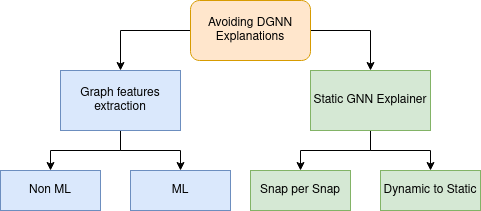
\includegraphics[width = 355pt]{Thesis_group_report_template_liris_en/Images/Avoiding DGNN Explainability Diagram.drawio.png}
    \caption{Avoiding dynamic GNN explainers} \label{fig:image}
    \label{other expl}
\end{figure}

1)static explainer working for Dynamic Graphs
2) Dynamic graphs changing graph into static one then static explainer
3)specific dy graphs explainer (table lit review 2) (not much anomaly detection...
4)graph features (topology,time) into classic ML
5)non ML --> stat, similarity in Time series,...

Figure~\ref{other expl} epxlain the figure...

+Table https://docs.google.com/document/d/1HVIT7x49c-3vlMisJMwkZ8TXNDjx-cXolEflYzA7QLw/edit explain...

\subsection{Application on Fraud transaction}

\subsubsection{Fraud detection}
DyHGN,xFraud,EvolveGCN
3 datasets

\subsubsection{Fraud explanation}
GNNExplainer+... (xFraud) static
XGBoost (DyHGN)

conclusion: use Perturbation methods better for 1) Anomaly detection 2) temporal (me lstm embeddings)
and/or similarity btw Time Series (DTW) similarity= explanation

\clearpage

%
% ---- Discussion ----
%
\section{Discussion \& Critical Reflection}
Discuss the results of your analysis here. Critically reflect on your analysis and the results. Discuss the limitations of your analysis, the impact these limitations have on your results and provide solutions.



\subsection{Future Directions}
create an explainer for anomaly detection in Dynamic graphs (for expl EvolveGCN)
create data repo for temporal graphs
merge PyGeoTemp and Py GOD

REALLY cool stuff: Catching up to modern credit card fraud models but with real explainability... streaming live heterogenous graph data into dynamic [black-box] models, connected to timestep-aware explainers.

\subsection{Contribution}
1)A survey on explainability in Dynamic Graphs
2)Showing current shortcomings in performance and explainability (GNN vs ML, static vs dynamic, homegenous vs heterogenous) --> simple often better
3) Help to create a new explainer for anomaly detection in dynamic graph ( 3 datasets, survey, advices,...)

\clearpage


%
% ---- Conclusion ----
%
\section{Conclusion}
Place the conclusion here. Summarize the methodology, results and the main takeaways.

\clearpage

%
% ---- Bibliography ----
%
% Add your references to the file 'mybibliography.bib'. Then cite the references with the following command: \cite.
%
% BibTeX users should specify bibliography style 'splncs04'.
% References will then be sorted and formatted in the correct style.
\bibliographystyle{splncs04}
\bibliography{Thesis_group_report_template_liris_en/bibliography-zotero} \label{references}
%
%
\clearpage
% ---- Appendices ----
%
\section*{Appendix}
\addcontentsline{toc}{section}{Appendix}
\input{Content/7_Appendix.tex}
\clearpage

%
% ---- List of figures ----
%
\listoffigures
\clearpage
%
% ---- List of tables ----
%
\listoftables

\cleardoublepage

\end{document}
